\documentclass[14pt,titlepage, a4paper]{extarticle}
\usepackage{tikz}
\usepackage{pgfplots}
\usetikzlibrary{shapes.geometric, arrows, positioning}
\usepackage{multicol}
\usepackage{minted}
\usepackage[a4paper, margin=0.5in]{geometry}
% tikz styling
\tikzstyle{block} = [rectangle, 
			draw, 
			rounded corners, 
			text centered, 
			minimum height = 2em]
\tikzstyle{rect} = [rectangle, 
			draw, 
			text centered, 
			minimum height = 2em]
\tikzstyle{nrect} = [rectangle, 
			text centered, 
			minimum height = 2em]
\tikzstyle{line} = [draw, -latex']
\tikzstyle{cloud} = [draw, ellipse, minimum height=2em]

\title{Networks Lab Report\\Assignment 3}
\author{Md Sahil\\BCSE III\\Roll-001710501029}
\date{}

\begin{document}

{\maketitle}

\section{Objective}
To implement 1-persistent, non-persistent and p-persistent CSMA techniques.

\section{Design and Implementation}

\subsection{Program structure}
The implementation is done using sockets.
The clients and server communicate with each other using sockets.
Listening on the channel is done through a separate 
thread (for both client and server).
There can be multiple client instances. All the clients are connected to the
central server. The cental server holds the channel(a buffer).


\subsubsection{The Server class}
The server class instance acts as a medium to connect two clients. 
Whenever the server is starts listening and accepting client socket
connections. Each time a client connection is made, its control is
passed on to the client handler thread. The client handler thread then 
listens for incoming frames from the assigned client socket.
The server also maintains a list of mappings of clients with port 
numbers and client addresses. When ever a client tries to connect to a server. 
The server maps the port number with the client address.
When a client tries to sent messages to another client, the server checks the
destination address of the message, finds the port mapped to the address
and forwards the message to the destination client.
The server holds the incomming messages in a buffer, which acts as the channel here.
When ever a new packet arrives and the buffer is non empty, a collision is registered.
\par\null\par
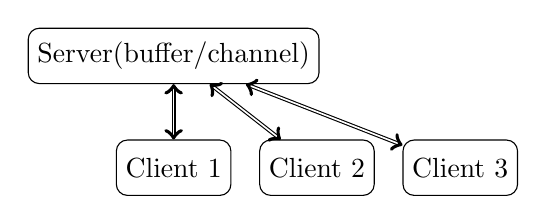
\begin{tikzpicture}[node distance = 1em, auto]
	\node [block] (server) {Server(buffer/channel)};
	\node [block, below=2em of server] (client1) {Client 1};
	\node [block, right=of client1] (client2) {Client 2};
	\node [block, right=of client2] (client3) {Client 3};
	\draw [double,<->] (server) -- (client1);
	\draw [double,<->] (server) -- (client2);
	\draw [double,<->] (server) -- (client3);
\end{tikzpicture}

\subsubsection{The Client class}
The instances of Client class acts as stations. It has 3 functions 
\emph{onePersistent()}, \emph{nonPersistent()} and \emph{pPersistent()}.
Each function implements its corresponding CSMA technique.

\par\null\par
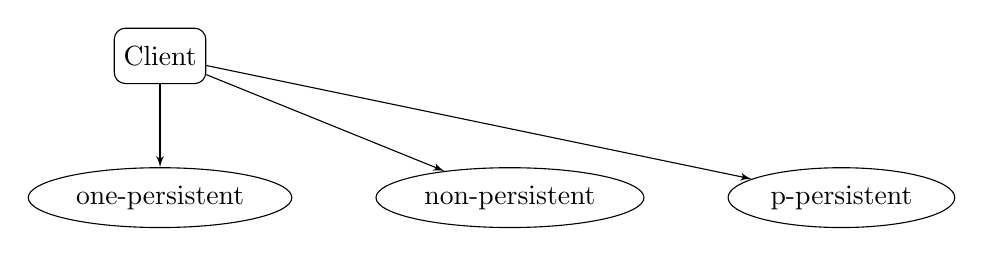
\begin{tikzpicture}[node distance = 3em, auto]
	\node [block] (clientClass) {Client};
	\node [cloud, below=of clientClass] (one) {one-persistent};
	\path [line] (clientClass) -- (one);
	\node [cloud, right=of one] (non) {non-persistent};
	\path [line] (clientClass) -- (non);
	\node [cloud, right=of non] (p) {p-persistent};
	\path [line] (clientClass) -- (p);
\end{tikzpicture}



\section{Code snippets}
\subsection{Server}
\begin{minted}[%
breaklines,
mathescape,
linenos,
numbersep=5pt,
frame=single,
numbersep=5pt,
xleftmargin=0pt,
fontsize=\footnotesize,
obeytabs=true,
tabsize=2,
]{java}
package dllp;

import java.io.*;
import java.net.ServerSocket;
import java.net.Socket;
import java.util.*;

/**Frame format:
 * 1 byte premble
 * 1 bytes destination address
 * 1 bytes source address
 * 1 - 10 bytes of data
 *
 *
 * If the premble is set to 00000000 then it is for dhcpLite request
 * If the premble is set to 00000001 then it is for dhcpLite granted
 * If the premble is set to 00000010 then it is for dhcpLite rejected
 * If the premble is set to 10000000 then it is for data transfer
 */

public class Server {

	public static final String DHCPLITE_REQUEST 	= "00000000";
	public static final String DHCPLITE_GRANTED 	= "00000001";
	public static final String DHCPLITE_REJECTED 	= "00000010";
	public static final String DATA_TRANSFER 	= "10000000";
	public static final double ERROR_P 		= 0.3;

	private static Map<String, ClientHandler> dns = new HashMap<String, ClientHandler>();

	private static class ClientHandler implements Runnable {
		private Socket soc;
		public PrintWriter out;
		public BufferedReader in;

		public ClientHandler(Socket s) {
			soc = s;
			try {
				out = new PrintWriter(soc.getOutputStream(), true);
				in = new BufferedReader(
					new InputStreamReader(
						soc.getInputStream()
						)
					);
			} catch (IOException e) {
				e.printStackTrace();
				System.exit(0);
			}
		}

		public void dataTranser(String msg) {
			/**Function for data tranfer between clients 
			 * void dataTranser(String message_to_be_send)
			 * */
			String destination = msg.substring(8,16);
			String source = msg.substring(16,24);
			double p = Math.random();
			if(p>ERROR_P) {
				dns.get(destination).out.println(msg);
				System.out.println("Message passed from:"
						+ source
						+ " to:"
						+ destination);
			} else {
				System.out.println("Error while passing message from:"
						+ source
						+ " to:"
						+ destination);
			}
		}

		public void dhcpLite(String msg) {
			/**Function mac address registration on server
			 * void dhcpLite(String dhcp_message_received_from_server)
			 * */
			try {
				String mac_addr = msg.substring(8,16);
				if(dns.containsKey(mac_addr)) {
					out.println(DHCPLITE_REJECTED);
					soc.close();
				} else {
					dns.put(mac_addr,this);
					out.println(DHCPLITE_GRANTED);
					System.out.println("Connection established with:" 
							+ mac_addr 
							+ " at socket:" 	
							+ soc.getRemoteSocketAddress().toString());
				}
			} catch (StringIndexOutOfBoundsException e) {
				System.out.println("Socket:"
						+ soc.getRemoteSocketAddress()
						+ " Requested an invalid mac_address registration");
				out.println(DHCPLITE_REJECTED);
			} catch (Exception e) {
				e.printStackTrace();
				System.exit(0);
			}
		}

		public void run() {
			System.out.println("Attempting to connect:" 	
					+ soc.getRemoteSocketAddress().toString());

			/** starts listeining to client indefinitely */ 
			try {
				while(!soc.isClosed()) {
					if(in.ready()) {
						String msg = in.readLine();
						//System.out.println("Received:" + msg);
						if(msg.substring(0,8).equals(DHCPLITE_REQUEST))
							dhcpLite(msg);
						else if(msg.substring(0,8).equals(DATA_TRANSFER)) {
							//System.out.println("Data:" + msg);
							dataTranser(msg);
						}
						else
							System.out.println("Unknown premble:" + msg.substring(0,8));
					}
				}
			} catch (IOException e) {
				e.printStackTrace();
				System.exit(0);
			}
		}
	}

	public static int PORT = 8888;
	public static void run() {
		try {
			ServerSocket serversocket = new ServerSocket(PORT);
			System.out.println("Server Started!");	
			while(true) {
				Socket soc = serversocket.accept();
				new Thread(new ClientHandler(soc)).start();
			}
			//serversocket.close();
		} catch (IOException e) {
			e.printStackTrace();
		}
	}


	public static void main(String[] args) {
		run();
	}
}
\end{minted}

\subsection{Client}
\begin{minted}[%
breaklines,
mathescape,
linenos,
numbersep=5pt,
frame=single,
numbersep=5pt,
xleftmargin=0pt,
fontsize=\footnotesize,
obeytabs=true,
tabsize=2,
]{java}
import java.util.Random;

public class Client {
	public static class ClientWrapper extends ClientClass {
		public ClientWrapper() {
			super();
		}

		protected void receiveMsg(String msg) {
			//do nothing for now
		}	

		protected void bufferUpdate(String buffer) {
		int newbufferStatus = Integer.parseInt(buffer,2);
		if(newbufferStatus != bufferStatus) {
				bufferStatus = newbufferStatus;
			}
		}

        protected String makeSequenceString (int n) {
	    	String sq = Integer.toBinaryString(n);
		    if(sq.length() > 8)
				sq = sq.substring(sq.length() - 8);
			else if(sq.length() < 8)
				while(sq.length()!=8)
					sq = "0" + sq;
			return sq;
		}

		protected void onePersitent() {
			int count = 0;
			while(true) {
				if(bufferStatus == 0) {
					try {
						String msg = makeSequenceString(count);
						System.out.println("Sending broadcast message:" + count);
						sendMsg(msg,BROADCAST_ADDRESS);
						count++;
						bufferStatus = 100;
						Thread.sleep(1000);
					} catch (Exception e) {
						e.printStackTrace();
						System.exit(0);
					}
				} else if(bufferStatus > 0) {
					System.out.print("");
				}

				if(count==100)
					break;
			}
		}


		protected void nonPersitent() {
			Random rand = new Random();
			int count = 0;
			while(true) {
				try {
					System.out.print("");
					if(bufferStatus == 0) {
						String msg = makeSequenceString(count);
						System.out.println("Sending broadcast message:" + count);
						sendMsg(msg,BROADCAST_ADDRESS);
						count++;
						bufferStatus = 100;
						Thread.sleep(1000);
					} else {
						System.out.print("");
						int n = rand.nextInt(2000);
						Thread.sleep(n);
					}
				} catch (Exception e) {
					e.printStackTrace();
					System.exit(0);
				}

				if(count==100)
					break;
			}
		}
		
		
		protected void pPersitent() {
			Random rand = new Random();
			int count = 0;
			while(true) {
				try {
					String msg = makeSequenceString(count);
					System.out.println("Sending broadcast message:" + count);
					int k = 0;
					double p = 0.5;
					int slottime = 1200;
					while(k<15) {
						if(bufferStatus == 0) {
							if(p<Math.random()) {
								sendMsg(msg,BROADCAST_ADDRESS);
								count++;
								//bufferStatus = 100;
								Thread.sleep(1000);
								break;
							} else {
								Thread.sleep(slottime);
							}
						} else if(bufferStatus>0) {
							System.out.print("");
							k++;
							int n = rand.nextInt((int)Math.pow(2.0,k+1));
							System.out.println("Backoff:" + n);
							Thread.sleep(n);
						}

						if(k>15) {
							System.out.println("Backing off limit reached, dumping packed");
							count++;
							break;
						}
					}
				} catch (Exception e) {
					e.printStackTrace();
					System.exit(0);
				}

				if(count==100)
					break;
			}
		}

		public void run(String mac_addr, String algo) {
			super.run(mac_addr);
			if(algo.equals("1"))
				onePersitent();
			else if(algo.equals("n"))
				nonPersitent();
			else if(algo.equals("p"))
				pPersitent();
			else {
				System.out.println("Invalid arguement!");
				System.exit(0);
			}
		}


	}

	public static void main(String args[]) {
		new ClientWrapper().run(args[0], args[1]);
	}
}
\end{minted}


\section{Results}
Observations have been taken by sending 100 packets from each station.

\begin{table}[!ht]
	\caption{With 2 stations}
	\bigskip
	\begin{tabular}{|l|l|l|l|l|l|l|}
		\hline
		&
		\multicolumn{2}{|l|}{one-persisent} & 
		\multicolumn{2}{|l|}{non-persisent} & 
		\multicolumn{2}{|l|}{p-persisent}\\
		\hline
		Sender &
		Throughput & Efficiency & 
		Throughput & Efficiency & 
		Throughput & Efficiency \\ 
		\hline
		1 & 
		0.9459 & 0.72 &
		0.2996 & 1.00 & 
		0.2504 & 1.00\\
		\hline
		2 &
		0.9458 & 0.62 & 
		0.2710 & 0.99 
		& 0.2465 & 0.99\\
		\hline
	\end{tabular}
\end{table}

\begin{table}[!ht]
	\caption{With 3 stations}
	\bigskip
	\begin{tabular}{|l|l|l|l|l|l|l|}
		\hline
		&
		\multicolumn{2}{|l|}{one-persisent} & 
		\multicolumn{2}{|l|}{non-persisent} & 
		\multicolumn{2}{|l|}{p-persisent}\\
		\hline
		Sender &
		Throughput & Efficiency & 
		Throughput & Efficiency & 
		Throughput & Efficiency \\ 
		\hline
		1 &
		0.8748 & 0.46 &
		0.2658 & 0.99 &
		0.1804 & 1.00\\
		\hline
		2 &
		0.8663 & 0.49 & 
		0.2490 & 1.00 &
		0.1711 & 0.99\\
		\hline
		3 &
		0.8505 & 0.52 &
		0.2342 & 0.99 &
		0.1697 & 0.99\\
		\hline
	\end{tabular}
\end{table}

\begin{table}[!ht]
	\caption{With 4 stations}
	\bigskip
	\begin{tabular}{|l|l|l|l|l|l|l|}
		\hline
		&
		\multicolumn{2}{|l|}{one-persisent} & 
		\multicolumn{2}{|l|}{non-persisent} & 
		\multicolumn{2}{|l|}{p-persisent}\\
		\hline
		Sender &
		Throughput & Efficiency & 
		Throughput & Efficiency & 
		Throughput & Efficiency \\ 
		\hline
		1 &
		0.6447 & 0.35 &
		0.1980 & 0.93 & 
		0.1841 & 0.98\\
		\hline
		2 & 
		0.6196 & 0.34 &
		0.1962 & 0.97 & 
		0.1712 & 0.99\\
		\hline
		3 &
		0.6197 & 0.47 &
		0.1891 & 0.95 & 
		0.1816 & 0.99\\
		\hline
		4 &
		0.6157 & 0.37 & 
		0.1852 & 0.95 & 
		0.1555 & 0.97\\
		\hline
	\end{tabular}
\end{table}

\subsection{One-persisent}
\begin{tikzpicture}
\begin{axis}[name=oneeff,
	xlabel = {no of stations},
	ylabel = {Efficiency},
	ymin = 0,
	ymax = 1,
	xtick = {2,3,4}] 
	\addplot[color=red, nodes near coords, mark=x] 
	table{./data/1_efficiency};
\end{axis}	
\end{tikzpicture}
\null
\begin{tikzpicture}
\begin{axis}[name=oneput,
	xlabel = {no of stations},
	ylabel = {Throughput}, 
	xtick = {2,3,4}] 
	\addplot[color=red, nodes near coords, mark=x] 
	table{./data/1_throughput};
\end{axis}	
\end{tikzpicture}

\subsection{Non-persisent}
\begin{tikzpicture}
\begin{axis}[name=oneeff,
	xlabel = {no of stations},
	ylabel = {Efficiency},
	ymin = 0,
	xtick = {2,3,4}] 
	\addplot[color=red, nodes near coords, mark=x] 
	table{./data/n_efficiency};
\end{axis}	
\end{tikzpicture}
\null
\begin{tikzpicture}
\begin{axis}[name=oneput,
	xlabel = {no of stations},
	ylabel = {Throughput}, 
	xtick = {2,3,4}] 
	\addplot[color=red, nodes near coords, mark=x] 
	table{./data/n_throughput};
\end{axis}	
\end{tikzpicture}

\subsection{p-persisent}
For The following graphs we keep the value of \emph{p} at 0.5 and
vary the number of stations.
\\

\noindent
\begin{tikzpicture}
\begin{axis}[name=oneeff,
	xlabel = {no of stations},
	ylabel = {Efficiency},
	ymin = 0,
	xtick = {2,3,4}] 
	\addplot[color=red, nodes near coords, mark=x] 
	table{./data/p_efficiency};
\end{axis}	
\end{tikzpicture}
\null
\begin{tikzpicture}
\begin{axis}[name=oneput,
	xlabel = {no of stations},
	ylabel = {Throughput}, 
	xtick = {2,3,4}] 
	\addplot[color=red, nodes near coords, mark=x] 
	table{./data/p_throughput};
\end{axis}	
\end{tikzpicture}

\noindent
For the following graphs we keep the number of stations fixed at 3 and
vary the value of \emph{p}.
\\
\begin{tikzpicture}
\begin{axis}[name=oneeff,
	xlabel = {p},
	ylabel = {Efficiency},
	ymin = 0,
	xtick = {0.2,0.5,0.8}] 
	\addplot[color=red, nodes near coords, mark=x] 
	table{./data/pp_efficiency};
\end{axis}	
\end{tikzpicture}
\null
\begin{tikzpicture}
\begin{axis}[name=oneput,
	xlabel = {p},
	ylabel = {Throughput}, 
	xtick = {0.2,0.5,0.8}] 
	\addplot[color=red, nodes near coords, mark=x] 
	table{./data/pp_throughput};
\end{axis}	
\end{tikzpicture}

\pagebreak
\section{Comments}
\begin{itemize}
		\item The architecture of the code here is identical 
			to the previous assignment. 
		\item I faced some thread scheduling problems.
			For example in certain infinite while loops, adding a blank print statement
			changed the execution.
\end{itemize}

\end{document}
